\pagebreak
\subsection{Failure Analysis}\label{sec:failureanalysis}
During the flight the experiment experienced unexpected errors. This section will go into the procedures and results of the failure analysis. In general there was two stages of analysis, firstly the post flight analysis that was made as soon as the experiment was retrieved during campaign and, secondly the lab analysis that was made in the lab some time after launch campaign.

\subsubsection{Post flight analysis}
Shortly after the conclusion of failure on the AAC system an investigation plan was created to make sure that the team did not destroy any potential evidence. Deducted from the behaviour during flight, a list of potential problems was made and can be seen in Table \ref{tab:potential-failure-causes}. Most possible causes were unlikely due to the extensive testing made before flight.
\begin{table}[H]
    \centering
    \begin{tabular}{|c|c|}
    \hline
        1 & Shorted output pin on Arduino \\ \hline 
        2 & Pump elastic diaphragm broke \\ \hline 
        3 & Pump too cold \\ \hline 
        4 & Short circuit in pump\\ \hline 
        5 & Pump MOSFET broken\\ \hline 
        6 & Pump current draw too high\\ \hline 
        7 & Pump drive shaft blocked\\ \hline 
        8 & Pump tubing blocked\\ \hline 
    \end{tabular}
    \caption{List of Potential Failure Causes}
    \label{tab:potential-failure-causes}
\end{table}



Shortly after the experiment was retrieved a structured post flight investigation was made to investigate the possible causes of the in flight failure. The experiment walls were removed one at a time and there was no unexpected smells when opening the walls of the experiment that might have indicated burning of components. After the main PCB board was accessible, resistance measurements were taken on the MOSFET's. Which all were the same, indicating that the MOSFET's were not damaged. There were no shorts anywhere on the PCB either. The forward resistance of the pump was measured and compared to the forward resistance of a spare pump. The resistances were similar and deemed not to be suspicious. There was no discontinuities on the PCB where they were not expected. No problems were found from electrical measurements and visual inspection. 

Thus the next step in the procedure was to try to start the system from a power supply and check functionality. The power supply was set to 28.8V and a current limit of 1.8A. The system was turned on and data was feed out nominally as it did during flight as well. After inspecting basic functionality of the experiment the pump and the flushing valve were turned on and opened to see if the same issue occurred as during flight. The pump turned on and the valve opened nominally and pumped air through the system. Since the pipes going out were dismounted at this point and one of the concerns was that the pump might have been blocked, the inlet of the pump was blocked and the procedure repeated. The pump turned on again, although without blowing air, as expected.

At this point the team had suspicions that it might be a current limitation problem since the same behaviour has been seen before in the lab when the experiment could not be supplied with enough current. Thus a decision was made to change the settings of the bench power supply used during testing. It was first set to 24V and 1.8A current limitation and the experiment continued to work nominally. Next, the power supply was set to 24V and 1A and the pump could no longer start at this point and the exact same behaviour as during flight was seen. The system shut down, stopped sending data to the ground station, then rebooted and reestablished the telemetry feed. At this point, no further testing was made at the campaign due to others needing the used facilities and it was deemed safe to continue the testing in the lab later on.

\subsubsection{Lab analysis}
The lab analysis mainly focused on the power consumption of the pump and what happened power wise when the pump was turned on. The whole system was powered through a bench power supply with a 206m Ohm resistance in series to be able to measure the peak currents when the pump turns on by measure the voltage drop over this resistance with an oscilloscope. There were two notable peaks when starting the pump, the first was on a time scale of 100ms and produced a total current draw of 1.019A. The second was on the time scale of 110$\micro$s and had a total current draw of 7.56A. Although, it is not certain that the second peak is real, it could have been produced by other disturbances since similar behaviours have been seen before on the same scope when other devices on the power net have been turned on or off.

After these test were performed, the experiment was tested with a test battery pack consisting of eight SAFT LSH20 cells. Although, the specific cells tested with had already been used and it is known that these batteries self drain once they have been used once. When trying to start the pump, the same behaviour as during flight failure was seen. Furthermore the voltage on the batteries dropped drastically to 3.5V from 22.9V which would explain the system shutdown. This can be seen in Figure \ref{fig:experiment-battery-test}.

\begin{figure}[H]
    \centering
    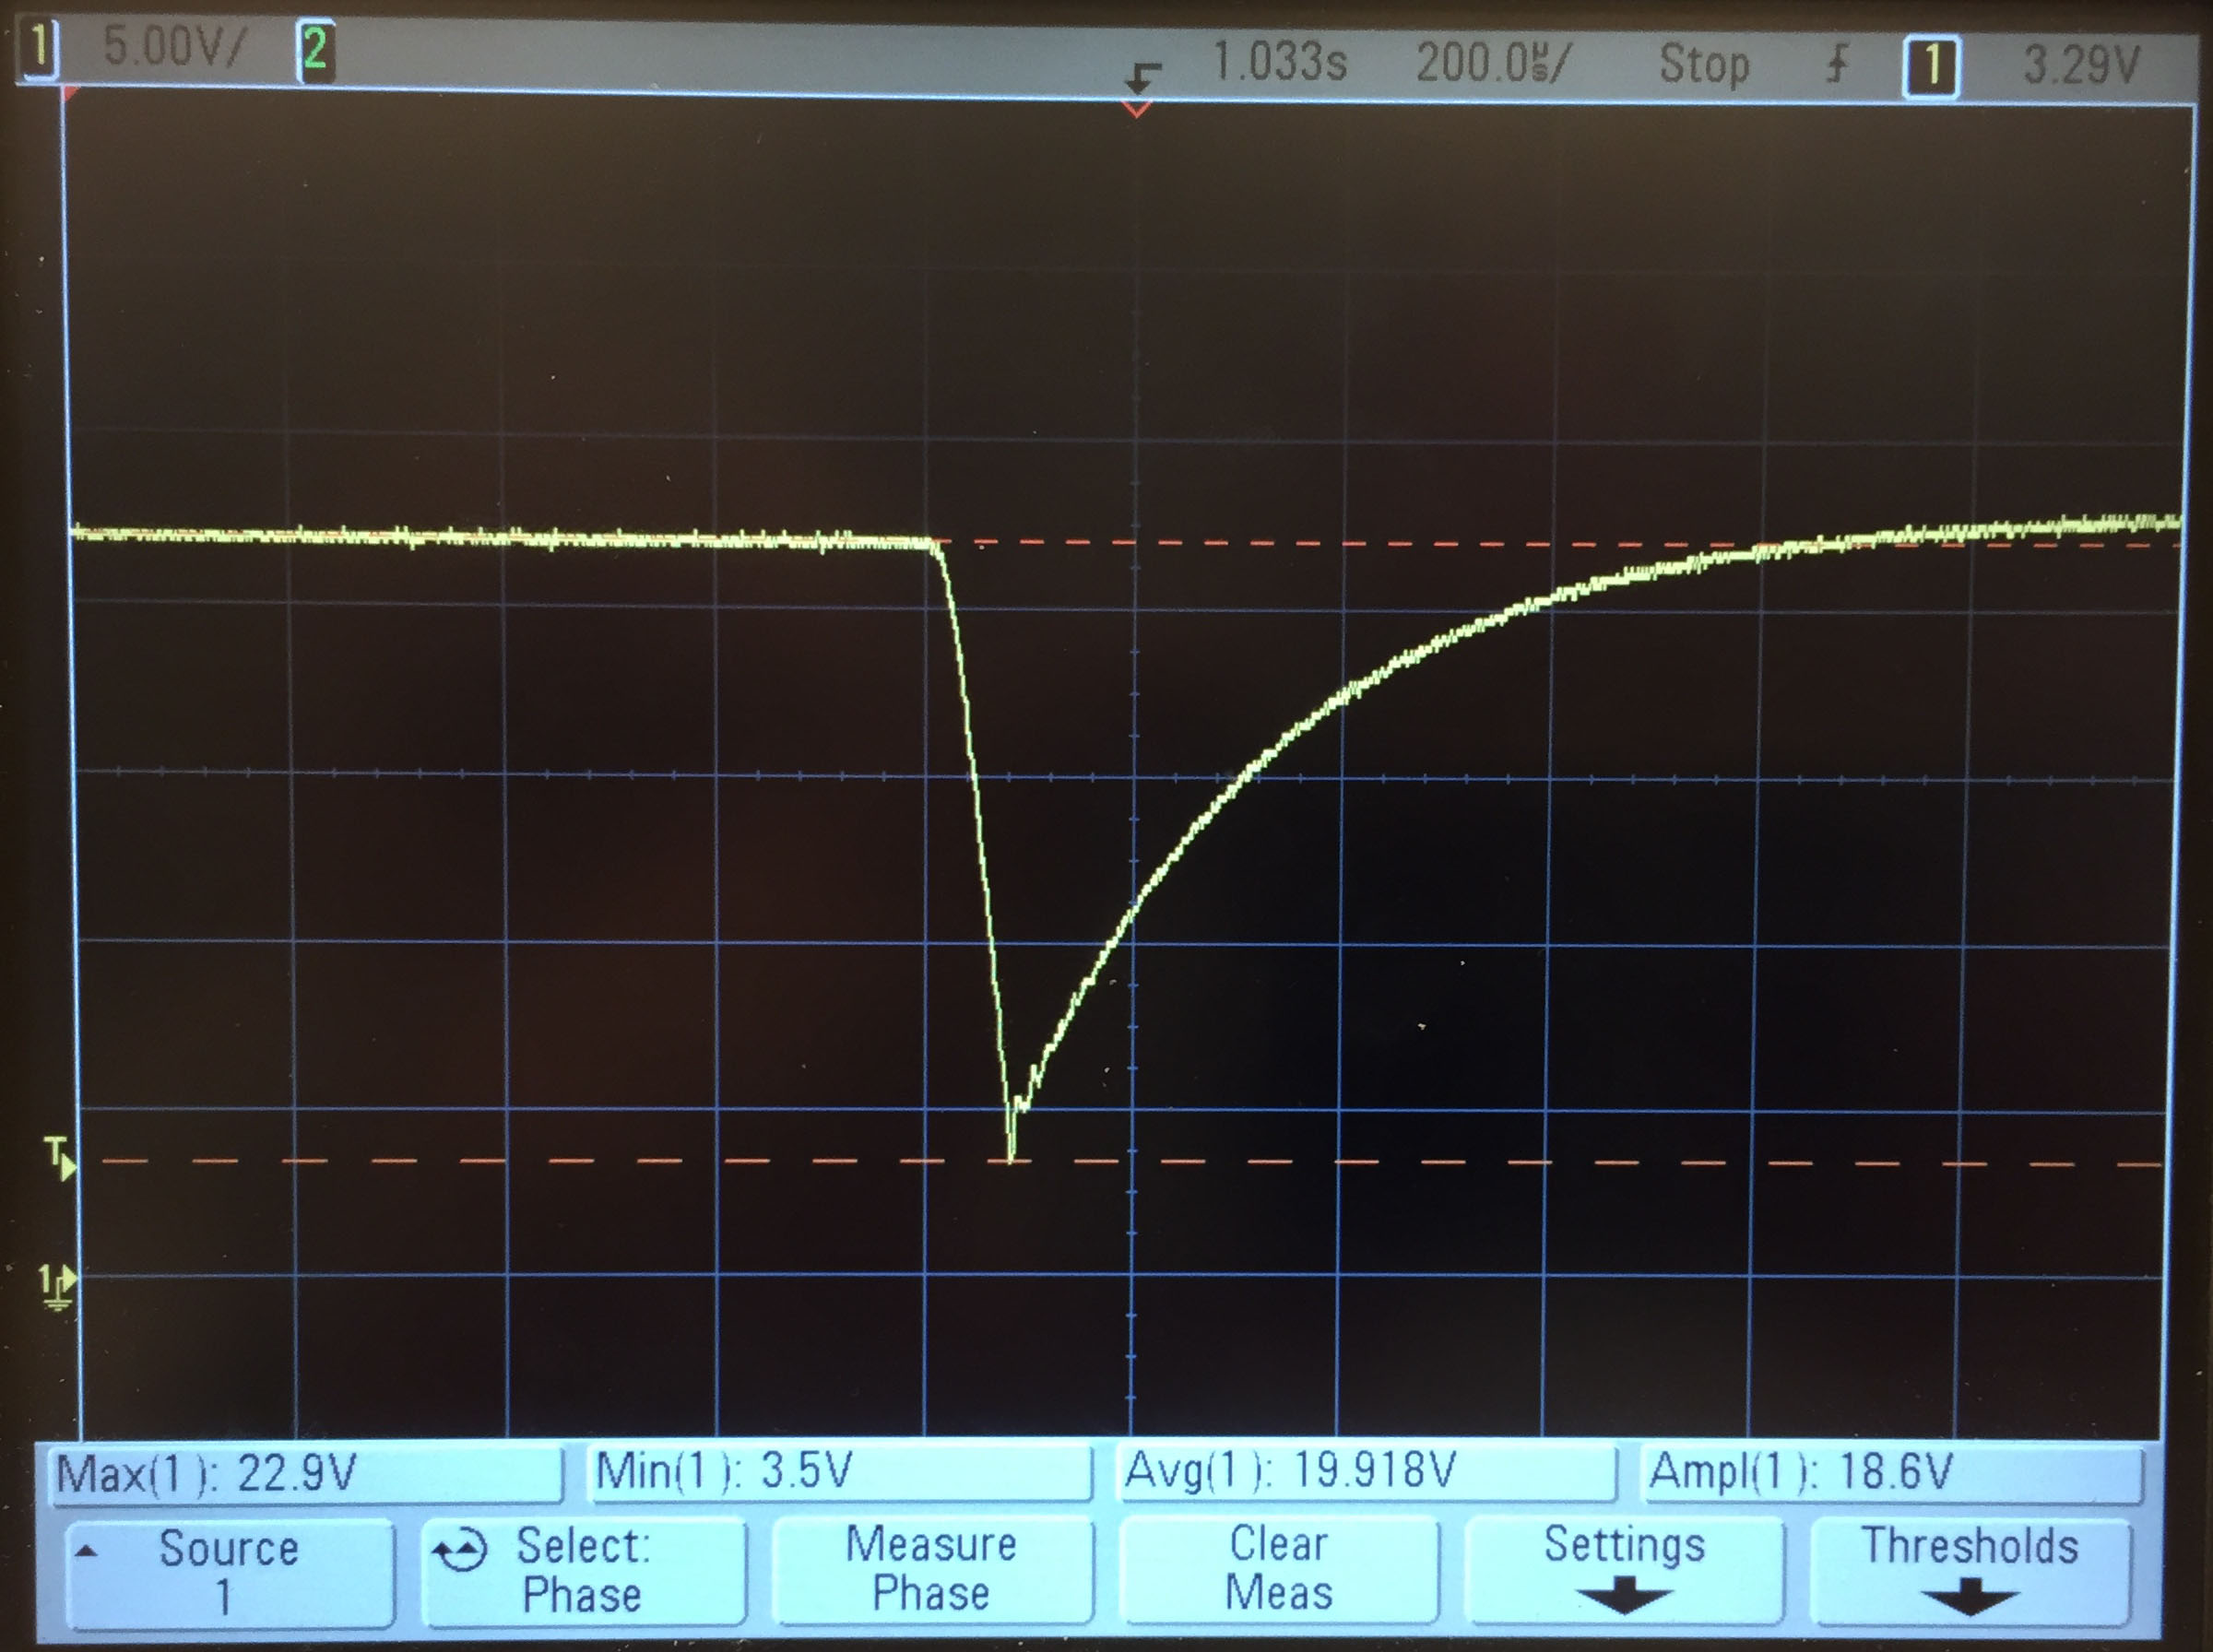
\includegraphics[width=0.6\textwidth]{7-data-analysis-and-results/img/BatteryTestPumpStart.JPG}
    \caption{Supply Voltage During Pump Start While Running on Batteries}
    \label{fig:experiment-battery-test}
\end{figure}

\subsubsection{Conclusion}
The experiment works within the current specifications of a single SAFT LSH20 cell. Although, the supplier has not specified the single cell behaviour for short peaks such as ~100$\micro$s. The effects on current specifications when using these cells in series is also unknown. Although, it is known that lithium-thionyl chloride batteries have a relatively large internal resistance which might affect the performance. Thus the conclusion is that the experiment was current limited and thus reset itself, but the source of limitation is still unknown. 

Since it was not possible to start the pump during the pre-flight readiness review as a result of the flushing already being made, starting the pump while running on batteries should have been tested before. Either in the Lab, or before the system was flushed at launch campaign. Then the issue might have been discovered before the flight.